
\chapter{Getting Started}


\section{A C++ TANGO client}

\noindent The quickest way of getting started is by studying this
example :


\begin{minted}[linenos]{cpp}
/* 
 * example of a client using the TANGO C++ api.
 */
#include <tango.h>
using namespace Tango;
int main(unsigned int argc, char **argv)
{
    try
    {

//
// create a connection to a TANGO device
//
 
        DeviceProxy *device = new DeviceProxy("sys/database/2");
 
//
// Ping the device
//
 
        device->ping();
 
//
// Execute a command on the device and extract the reply as a string
//
 
        string db_info; 
        DeviceData cmd_reply;
        cmd_reply = device->command_inout("DbInfo");
        cmd_reply >> db_info;
        cout << "Command reply " << db_info << endl;
 
//
// Read a device attribute (string data type)
//
 
        string spr;
        DeviceAttribute att_reply;
        att_reply = device->read_attribute("StoredProcedureRelease");
        att_reply >> spr;
        cout << "Database device stored procedure release: " << spr << endl;
    }
    catch (DevFailed &e)
    {
        Except::print_exception(e);
        exit(-1);
    } 
}
\end{minted}


\noindent Modify this example to fit your device server or client's
needs, compile it and link with the library -ltango. Forget about
those painful early TANGO days when you had to learn CORBA and manipulate
Any's. Life's going to easy and fun from now on !


\section{A TANGO device server}

The code given in this chapter as example has been generated using
POGO. Pogo\index{Pogo} is a code generator for Tango device server.
See \cite{Pogo doc} for more information about POGO. The following
examples briefly describe how to write device class with commands
which receives and return different kind of Tango data types and also
how to write device attributes\index{attribute} The device class
implements 5 commands and 3 attributes. The commands are :
\begin{itemize}
\item The command \textbf{DevSimple} deals with simple Tango data type
\item The command \textbf{DevString} deals with Tango strings
\item \textbf{DevArray} receive and return an array of simple Tango data
type
\item \textbf{DevStrArray} which does not receive any data but which returns
an array of strings
\item \textbf{DevStruct} which also does not receive data but which returns
one of the two Tango composed types (DevVarDoubleStringArray)
\end{itemize}
For all these commands, the default behavior of the state machine
(command always allowed) is acceptable. The attributes are :
\begin{itemize}
\item A spectrum type attribute of the Tango string type called \textbf{StrAttr}
\item A readable attribute of the Tango::DevLong type called \textbf{LongRdAttr}.
This attribute is linked with the following writable attribute
\item A writable attribute also of the Tango::DevLong type called \textbf{LongWrAttr}.
\end{itemize}
Since release 9, a Tango device also supports pipe. This is an advanced
feature reserved for some specific cases. Therefore, there is no device
pipe example in this \textquotedbl{}Getting started\textquotedbl{}
chapter.


\subsection{The commands and attributes code}

For each command called DevXxxx, pogo generates in the device class
a method named dev\_xxx which will be executed when the command is
requested by a client. In this chapter, the name of the device class
is \emph{DocDs}


\subsubsection{The DevSimple command}

This method receives a Tango::DevFloat\index{Tango::DevFloat} type
and also returns a data of the Tango::DevFloat type which is simply
the double of the input value. The code for the method executed by
this command is the following:


\begin{minted}[linenos]{cpp}
     1  Tango::DevFloat DocDs::dev_simple(Tango::DevFloat argin)
     2  {
     3          Tango::DevFloat argout ;
     4          DEBUG_STREAM << "DocDs::dev_simple(): entering... !" << endl;
     5  
     6          //      Add your own code to control device here
     7  
     8          argout = argin * 2;
     9          return argout;
    10  }
\end{minted}


This method is fairly simple. The received data is passed to the method
as its argument. It is

doubled at line 8 and the method simply returns the result.


\subsubsection{The DevArray command}

This method receives a data of the Tango::DevVarLongArray\index{Tango::DevVarLongArray}
type and also returns a data of the Tango::DevVarLongArray type. Each
element of the array is doubled. The code for the method executed
by the command is the following :


\begin{minted}[linenos]{cpp}
     1  Tango::DevVarLongArray *DocDs::dev_array(const Tango::DevVarLongArray *argin)
     2  {
     3          //      POGO has generated a method core with argout allocation.
     4          //      If you would like to use a static reference without copying,
     5          //      See "TANGO Device Server Programmer's Manual"
     6          //              (chapter x.x)
     7          //------------------------------------------------------------
     8          Tango::DevVarLongArray  *argout  = new Tango::DevVarLongArray();
     9                  
    10          DEBUG_STREAM << "DocDs::dev_array(): entering... !" << endl;
    11  
    12          //      Add your own code to control device here
    13  
    14          long argin_length = argin->length();    
    15          argout->length(argin_length);
    16          for (int i = 0;i < argin_length;i++)
    17                  (*argout)[i] = (*argin)[i] * 2;
    18  
    19          return argout;
    20  }
\end{minted}


The argout data array is created at line 8. Its length is set at line
15 from the input argument length. The array is populated at line
16,17 and returned. This method allocates memory\index{memory} for
the argout array. This memory is freed by the Tango core classes after
the data have been sent to the caller (no delete is needed). It is
also possible to return data from a statically allocated array without
copying. Look at chapter \ref{Data exchange} for all the details.


\subsubsection{The DevString command}

This method receives a data of the Tango::DevString\index{Tango::DevString}
type and also returns a data of the Tango::DevString type. The command
simply displays the content of the input string and returns a hard-coded
string. The code for the method executed by the command is the following
:


\begin{minted}[linenos]{cpp}
     1  Tango::DevString DocDs::dev_string(Tango::DevString argin)
     2  {
     3          //      POGO has generated a method core with argout allocation.
     4          //      If you would like to use a static reference without copying,
     5          //      See "TANGO Device Server Programmer's Manual"
     6          //              (chapter x.x)
     7          //------------------------------------------------------------
     8          Tango::DevString        argout;
     9          DEBUG_STREAM << "DocDs::dev_string(): entering... !" << endl;
    10  
    11          //      Add your own code to control device here
    12  
    13          cout << "the received string is " << argin << endl;
    14          
    15          string str("Am I a good Tango dancer ?");
    16          argout = new char[str.size() + 1];
    17          strcpy(argout,str.c_str());
    18          
    19          return argout;
    20  }
\end{minted}


The argout string is created at line 8. Internally, this method is
using a standard C++ string. Memory for the returned data is allocated
at line 16 and is initialized at line 17. This method allocates memory\index{memory}
for the argout string. This memory is freed by the Tango core classes
after the data have been sent to the caller (no delete is needed).
It is also possible to return data from a statically allocated string
without copying. Look at chapter \ref{Data exchange} for all the
details.


\subsubsection{The DevStrArray command}

This method does not receive input data but returns an array of strings
(Tango::DevVarStringArray\index{Tango::DevVarStringArray} type).
The code for the method executed by this command is the following:


\begin{minted}[linenos]{cpp}
     1  Tango::DevVarStringArray *DocDs::dev_str_array()
     2  {
     3          //      POGO has generated a method core with argout allocation.
     4          //      If you would like to use a static reference without copying,
     5          //      See "TANGO Device Server Programmer's Manual"
     6          //              (chapter x.x)
     7          //------------------------------------------------------------
     8          Tango::DevVarStringArray        *argout  = new Tango::DevVarStringArray();
     9  
    10          DEBUG_STREAM << "DocDs::dev_str_array(): entering... !" << endl;
    11  
    12          //      Add your own code to control device here
    13  
    14          argout->length(3);
    15          (*argout)[0] = CORBA::string_dup("Rumba");
    16          (*argout)[1] = CORBA::string_dup("Waltz");
    17          string str("Jerck");
    18          (*argout)[2] = CORBA::string_dup(str.c_str());
    19          return argout;
    20  }
\end{minted}


The argout data array is created at line 8. Its length is set at line
14. The array is populated at line 15,16 and 18. The last array element
is initialized from a standard C++ string created at line 17. Note
the usage of the \emph{string\_dup\index{string-dup}} function of
the CORBA namespace. This is necessary for strings array due to the
CORBA memory\index{memory} allocation schema.


\subsubsection{The DevStruct command}

This method does not receive input data but returns a structure of
the Tango::DevVarDoubleStringArray\index{Tango::DevVarDoubleStringArray}
type. This type is a composed type with an array of double and an
array of strings. The code for the method executed by this command
is the following:


\begin{minted}[linenos]{cpp}
     1  Tango::DevVarDoubleStringArray *DocDs::dev_struct()
     2  {
     3          //      POGO has generated a method core with argout allocation.
     4          //      If you would like to use a static reference without copying,
     5          //      See "TANGO Device Server Programmer's Manual"
     6          //              (chapter x.x)
     7          //------------------------------------------------------------
     8          Tango::DevVarDoubleStringArray  *argout  = new Tango::DevVarDoubleStringArray();
     9  
    10          DEBUG_STREAM << "DocDs::dev_struct(): entering... !" << endl;
    11          
    12          //      Add your own code to control device here
    13  
    14          argout->dvalue.length(3);
    15          argout->dvalue[0] = 0.0;
    16          argout->dvalue[1] = 11.11;
    17          argout->dvalue[2] = 22.22;
    18          
    19          argout->svalue.length(2);
    20          argout->svalue[0] = CORBA::string_dup("Be Bop");
    21          string str("Smurf");
    22          argout->svalue[1] = CORBA::string_dup(str.c_str());
    23          
    24          return argout;
    25  }
\end{minted}


The argout data structure is created at line 8. The length of the
double array in the output structure is set at line 14. The array
is populated between lines 15 and 17. The length of the string array
in the output structure is set at line 19. This string array is populated
between lines 20 an 22 from a hard-coded string and from a standard
C++ string. This method allocates memory\index{memory} for the argout
data. This memory is freed by the Tango core classes after the data
have been sent to the caller (no delete is needed). Note the usage
of the \emph{string\_dup\index{string-dup}} function of the CORBA
namespace. This is necessary for strings array due to the CORBA memory
allocation schema.


\subsubsection{The three attributes\index{attribute}}

Some data have been added to the definition of the device class in
order to store attributes value. These data are (part of the class
definition) :


\begin{minted}[linenos]{cpp}
     1  
     2  
     3  protected :     
     4          //      Add your own data members here
     5          //-----------------------------------------
     6          Tango::DevString        attr_str_array[5];
     7          Tango::DevLong          attr_rd;
     8          Tango::DevLong          attr_wr;
\end{minted}


One data has been created for each attribute. As the StrAttr attribute
is of type spectrum with a maximum X dimension of 5, an array of length
5 has been reserved.

Several methods are necessary to implement these attributes. One method
to read the hardware which is common to all \textquotedbl{}readable\textquotedbl{}
attributes plus one \textquotedbl{}read\textquotedbl{} method for
each readable attribute and one \textquotedbl{}write\textquotedbl{}
method for each writable attribute. The code for these methods is
the following :


\begin{minted}[linenos]{cpp}
1 void DocDs::read_attr_hardware(vector<long> &attr_list)
2 {
3     DEBUG_STREAM << "DocDs::read_attr_hardware(vector<long> &attr_list) entering... "<< endl;
4 // Add your own code here
5 
6     string att_name;
7     for (long i = 0;i < attr_list.size();i++)
8     {
9         att_name = dev_attr->get_attr_by_ind(attr_list[i]).get_name();
10 
11        if (att_name == "LongRdAttr")
12        {
13            attr_rd = 5;
14        }
15    }
16 }
17 
18 void DocDs::read_LongRdAttr(Tango::Attribute &attr)
19 {
20     DEBUG_STREAM << "DocDs::read_LongRdAttr(Tango::Attribute &attr) entering... "<< endl;
21 
22     attr.set_value(&attr_rd);
23 }
24 
25 void DocDs::read_LongWrAttr(Tango::Attribute &attr)
26 {
27     DEBUG_STREAM << "DocDs::read_LongWrAttr(Tango::Attribute &attr) entering... "<< endl;
28 
29     attr.set_value(&attr_wr);
30 }
31 
32 void DocDs::write_LongWrAttr(Tango::WAttribute &attr)
33 {
34     DEBUG_STREAM << "DocDs::write_LongWrAttr(Tango::WAttribute &attr) entering... "<< endl;
35 
36     attr.get_write_value(attr_wr);
37     DEBUG_STREAM << "Value to be written = " << attr_wr << endl;
38 }
39 
40 void DocDs::read_StrAttr(Tango::Attribute &attr)
41 {
42     DEBUG_STREAM << "DocDs::read_StrAttr(Tango::Attribute &attr) entering... "<< endl;
43 
44     attr_str_array[0] = const_cast<char *>("Rock");
45     attr_str_array[1] = const_cast<char *>("Samba");
46 
47     attr_set_value(attr_str_array, 2);
48 }
\end{minted}


The \emph{read\_attr\_hardware\index{read-attr-hardware}()} method
is executed once when a client execute the read\_attributes\index{read-attributes}
CORBA request whatever the number of attribute to be read is. The
rule of this method is to read the hardware and to store the read
values somewhere in the device object. In our example, only the LongRdAttr
attribute internal value is set by this method at line 13. The method
\emph{read\_LongRdAttr()} is executed by the read\_attributes\index{read-attributes}
CORBA call when the LongRdAttr attribute is read but after the read\_attr\_hardware()
method has been executed. Its rule is to set the attribute value in
the TANGO core classes object representing the attribute. This is
done at line 22. The method \emph{read\_LongWrAttr()} will be executed
when the LongWrAttr attribute is read (after the \emph{read\_attr\_hardware()}
method). The attribute value is set at line 29. In the same manner,
the method called \emph{read\_StrAttr()} will be executed when the
attribute StrAttr is read. Its value is initialized in this method
at line 44 and 45 with the \emph{string\_dup\index{string-dup}} Tango
function. There are several ways to code spectrum or image attribute
of the DevString data type. A HowTo related to this topic is available
on the Tango control system Web site. The \emph{write\_LongWrAttr()}
method is executed when the LongWrAttr attribute\index{attribute}
value is set by a client. The new attribute value coming from the
client is stored in the object data at line 36.

Pogo also generates a file called \textquotedbl{}DocDsStateMachine.cpp\textquotedbl{}
(for a Tango device server class called DocDs). This file is used
to store methods coding the device state machine. By default a allways
allowed state machine is provided. For more information about coding
the state machine, refer to the chapter \textquotedbl{}Writing a device
server\textquotedbl{}.

\newpage{}

\vspace{5cm}


\begin{center}
\label{APicture}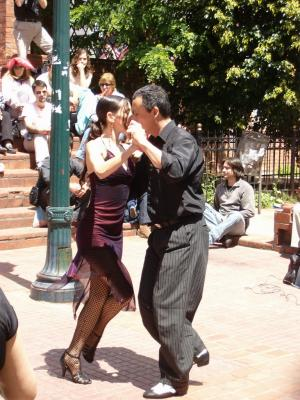
\includegraphics{dance/tg_argentine}
\par\end{center}
